\documentclass[10pt]{article}
% Submission (anonymous): \usepackage{tmlr}
% Camera-ready:            \usepackage[accepted]{tmlr}
% Preprint (arXiv):        \usepackage[preprint]{tmlr}
\usepackage[preprint]{tmlr}

\usepackage[T1]{fontenc}
\usepackage{hyperref}
\usepackage{url}
\usepackage{booktabs}
\usepackage{tabularx}
\usepackage{multirow}
\usepackage{graphicx}
\usepackage{amsmath,amssymb}
\usepackage{xcolor}
\usepackage{enumitem}
\usepackage{tikz}
\usetikzlibrary{positioning,arrows.meta,fit,calc}
\setlist{itemsep=1pt,topsep=3pt}

\newcommand{\ablCases}{6{,}660}
\newcommand{\ablFalseOk}{106}
\newcommand{\ablFalseOkOnly}{88}
\newcommand{\ablIncomplete}{2{,}328}
\newcommand{\ablInvisible}{1{,}617}
\newcommand{\ablInvisibleOnly}{1{,}230}
\newcommand{\ablMissing}{618}
\newcommand{\ablMissingOnly}{248}
\newcommand{\ablRSMiss}{1{,}230}
\newcommand{\ablRSMissPct}{53}
\newcommand{\ablRecallMiss}{1{,}710}
\newcommand{\ablRecallMissPct}{73}
\newcommand{\ablStatus}{375}
\newcommand{\ablStatusOnly}{374}
\newcommand{\adjSigList}{\texttt{crewai/events} $>$ \texttt{google-adk/otel}, \texttt{pydantic-ai/history} $>$ \texttt{pydantic-ai/otel}, \texttt{semantic-kernel/filters} $>$ \texttt{semantic-kernel/otel}, \texttt{semantic-kernel/otel} $>$ \texttt{smolagents/openinference}, \texttt{smolagents/openinference} $>$ \texttt{smolagents/memory}}
\newcommand{\allDropsPositive}{yes}
\newcommand{\bootReps}{2{,}000}
\newcommand{\bootScenarios}{103}
\newcommand{\coreCases}{660}
\newcommand{\coreComplete}{586}
\newcommand{\corePassed}{566}
\newcommand{\corePassedPct}{85.8}
\newcommand{\corePct}{88.8}
\newcommand{\curveHi}{51}
\newcommand{\curveLo}{83}
\newcommand{\dropMax}{.332}
\newcommand{\dropMin}{.042}
\newcommand{\dsCases}{11{,}544}
\newcommand{\dsEmitted}{58{,}906}
\newcommand{\eoAmbig}{1{,}866}
\newcommand{\eoDetected}{1{,}866}
\newcommand{\eoDetectedPct}{80.2}
\newcommand{\eoFalse}{2}
\newcommand{\eoMissed}{462}
\newcommand{\faAllTOne}{.943}
\newcommand{\faAllTOneLofo}{.870}
\newcommand{\faAllTThree}{.734}
\newcommand{\faAllTThreeLofo}{.718}
\newcommand{\faCountsTOne}{.829}
\newcommand{\faCountsTOneLofo}{.725}
\newcommand{\faNoMissingTTwo}{.975}
\newcommand{\faNoRatesTOne}{.947}
\newcommand{\faNoRatesTOneLofo}{.923}
\newcommand{\faNoRatesTThree}{.783}
\newcommand{\faNoRatesTThreeLofo}{.826}
\newcommand{\faNoRatesTTwo}{.976}
\newcommand{\faWithMissingTTwo}{.976}
\newcommand{\gbmTFourExact}{.701}
\newcommand{\gbmTOneF}{.947}
\newcommand{\gbmTThreeMacro}{.784}
\newcommand{\genCalls}{1{,}744}
\newcommand{\genCases}{6{,}000}
\newcommand{\genComplete}{3{,}746}
\newcommand{\genPct}{62.4}
\newcommand{\gtCases}{6{,}660}
\newcommand{\gtComplete}{4{,}332}
\newcommand{\gtIncomplete}{2{,}328}
\newcommand{\histFirst}{2025-03-29}
\newcommand{\histLast}{2026-10-03}
\newcommand{\iidGbmTOneMean}{.974}
\newcommand{\iidGbmTThreeMean}{.900}
\newcommand{\iidLrTOneMean}{.907}
\newcommand{\iidLrTThreeMean}{.700}
\newcommand{\iidTFourExact}{.910}
\newcommand{\iidTThreeMacro}{.892}
\newcommand{\llDetected}{1{,}098}
\newcommand{\llDetectedPct}{47.2}
\newcommand{\llFalse}{2}
\newcommand{\loDetected}{1{,}372}
\newcommand{\loDetectedPct}{58.9}
\newcommand{\loFalse}{1{,}696}
\newcommand{\loFalsePct}{39.2}
\newcommand{\loMissed}{956}
\newcommand{\lofoGbmTOneMean}{.923}
\newcommand{\lofoGbmTThreeMean}{.826}
\newcommand{\lofoLrTOneMean}{.757}
\newcommand{\lofoLrTThreeMean}{.657}
\newcommand{\lofoSdMax}{.441}
\newcommand{\lofoWorstExact}{.612}
\newcommand{\lofoWorstFw}{smolagents}
\newcommand{\logitCalls}{$-$0.32}
\newcommand{\logitCanc}{$-$0.70}
\newcommand{\logitNest}{$-$0.37}
\newcommand{\logitPar}{$-$1.23}
\newcommand{\logitRaise}{$-$0.50}
\newcommand{\logitRej}{$-$1.50}
\newcommand{\lrTFourExact}{.651}
\newcommand{\lrTThreeMacro}{.789}
\newcommand{\mutGenMin}{28}
\newcommand{\nAdj}{14}
\newcommand{\nAdjSig}{5}
\newcommand{\nSeeds}{3}
\newcommand{\nSurfaces}{15}
\newcommand{\nUnstable}{148}
\newcommand{\probeAll}{45.1}
\newcommand{\probeChance}{8.0}
\newcommand{\probeClasses}{15}
\newcommand{\probeCounts}{13.3}
\newcommand{\probeNoRates}{32.9}
\newcommand{\refClean}{yes}
\newcommand{\refCleanGen}{yes}
\newcommand{\seedNames}{1, 2, 3}
\newcommand{\seedSpread}{16}
\newcommand{\seqTOneHeld}{.911}
\newcommand{\seqTOneRandom}{.933}
\newcommand{\seqTThreeHeld}{.648}
\newcommand{\seqTThreeLofo}{.613}
\newcommand{\seqTThreeRandom}{.672}
\newcommand{\smolHi}{7}
\newcommand{\smolLo}{65}
\newcommand{\stableAgree}{5{,}852}
\newcommand{\stableAgreePct}{97.5}
\newcommand{\stableCases}{3{,}090}
\newcommand{\stableComplete}{2{,}304}
\newcommand{\stableFaithful}{2{,}980}
\newcommand{\stableFaithfulPct}{96.4}
\newcommand{\stablePct}{74.6}
\newcommand{\stressCases}{3{,}570}
\newcommand{\stressComplete}{2{,}028}
\newcommand{\stressPct}{56.8}
\newcommand{\tagMaxDiff}{.009}
\newcommand{\tagMaxDiffLofo}{.012}
\newcommand{\taskTestN}{2{,}832}
\newcommand{\taskTrainN}{5{,}884}
\newcommand{\taskValN}{2{,}344}
\newcommand{\tauCoreGen}{0.71}
\newcommand{\tauSeedMax}{0.80}
\newcommand{\tauSeedMean}{0.78}
\newcommand{\tauSeedMin}{0.77}
\newcommand{\tfTThreeHeld}{.705}
\newcommand{\tfTThreeRandom}{.729}
\newcommand{\totalMinutes}{47}

\makeatletter\newcommand{\inputtable}[1]{\@@input #1 }\makeatother
\newcommand{\todo}[1]{\textcolor{red}{[TODO: #1]}}
% Artifact links. For the anonymous submission, point these at an anonymized mirror.
\newcommand{\codeurl}{\url{https://github.com/pushkardg/tracegap}}
\newcommand{\dataurl}{\url{https://github.com/pushkardg/tracegap}}

\title{TraceGap: Measuring Whether LLM Agent Frameworks\\Record the Tool Calls Their Agents Make}

\author{\name Pushkar Devanahalli Gopalakrishna \email pushkar87dg@gmail.com}

\def\month{MM}
\def\year{YYYY}
\def\openreview{\url{https://openreview.net/forum?id=XXXX}}

\begin{document}
\maketitle

\begin{abstract}
Debugging, auditing, evaluation and training of LLM agents all consume the record that agent frameworks keep of tool calls, yet benchmarks for tool use evaluate whether \emph{models} call tools correctly, and to our knowledge none evaluates whether \emph{frameworks} record those calls correctly. We present TraceGap, a benchmark and dataset that drive agent frameworks with scripted models and compare each framework's own trace surface (callbacks, tracing spans, OpenTelemetry and OpenInference spans, events, message history) with ground truth that does not depend on the framework: the calls the model emitted and an execution ledger written by the tools themselves. Each case is scored for completeness and fidelity. Across nine widely used Python frameworks and fifteen trace surfaces, \coreComplete{} of \coreCases{} cases in 22 hand-written fault scenarios were complete (\corePct\%), and \genComplete{} of \genCases{} in a seeded generated suite (\genPct\%). Rankings use a Stable tier, defined by a structural rule that contained every verdict that varied across repeated runs; \stablePct\% of its \stableCases{} cases were complete, against \stressPct\% in the race-prone Stress tier. Failures concentrate in rejected calls, cancellation, failures inside parallel batches and nested agents, and a recall-only metric, the obvious first choice, would miss \ablRecallMissPct\% of them. A common pattern, span handling that does not see Python's cancellation exception, makes cancelled calls look successful in three frameworks, and in a fourth once another defect is fixed; TraceGap found defects in five frameworks, for which we provide fixes. A deliberately correct reference loop scores perfectly and eleven injected recording defects are each detected. An ablation shows that both ground-truth sources are needed: either alone misses or misreports a large share of failures. The released corpus of about 11{,}500 labeled cases defines four learning tasks; learned detectors of incomplete traces work well on the held-out test frameworks but vary widely across frameworks, classifying and reconstructing what was lost is harder, random splits substantially overestimate generalization compared with leave-one-framework-out evaluation, and features that identify the trace surface hurt it.
\end{abstract}

% =====================================================================
\section{Introduction}
\label{sec:intro}

LLM agents act through tools, and the record of those tool calls is what the rest of the stack consumes. Engineers debug from it, auditors review it, observability back ends aggregate it, trace-based evaluators and LLM judges score it~\citep{deshpande2025trail,zhang2025whowhen}, and trajectories collected from it become training data. That record is usually produced neither by the model nor by the application but by the \emph{agent framework}: LangGraph, the OpenAI Agents SDK, Pydantic AI, AutoGen and others expose callbacks, tracing spans, OpenTelemetry~\citep{otel2026genai} or OpenInference~\citep{openinference2026} spans, event streams and message histories. If a framework drops a call, reports a cancelled call as successful, or loses the calls of a run that failed, every consumer inherits the error without knowing it.

Benchmarks for tool use evaluate the model: whether it selects the right tool and arguments~\citep{patil2023gorilla,qin2024toolllm}, or completes tasks in interactive environments~\citep{yao2024tau,liu2024agentbench}. Work on agent traces analyses them, to localize agent errors~\citep{deshpande2025trail,cemri2025mast} or reconstruct provenance~\citep{wang2026survey}, and takes the recorded trace as correct. Yet an empirical study of LangChain and CrewAI found telemetry malfunctions among the root causes of framework bugs~\citep{zhu2026bugs}. The layer underneath has not been measured: \emph{given that a call happened, does the framework's trace say so, accurately?}

Measuring this is harder than it looks. Ground truth cannot come from the framework under test, real models make runs irreproducible, and the interesting conditions (a tool raising inside a batch of parallel calls, cancellation mid-call, a call to a tool that does not exist) are rare in natural traffic. TraceGap addresses these with scripted models, tools that write their own execution ledger, and fault scenarios that make rare conditions routine (Figure~\ref{fig:overview}).

\paragraph{Research questions.} We organize the study around six questions:
\begin{itemize}
\item[\textbf{RQ1}] How completely and faithfully do current agent frameworks record tool execution? (\S\ref{sec:results})
\item[\textbf{RQ2}] Under which execution conditions do surfaces fall short of the contract, and why? (\S\ref{sec:where}, \S\ref{sec:failures})
\item[\textbf{RQ3}] Are recording verdicts stable across repeated executions, and is the benchmark's design necessary? (\S\ref{sec:validation})
\item[\textbf{RQ4}] How has recording correctness changed across framework releases? (\S\ref{sec:history})
\item[\textbf{RQ5}] Can trace defects be detected from what a pipeline observes, without the execution ledger? (\S\ref{sec:data})
\item[\textbf{RQ6}] Do learned trace-defect detectors generalize to agent frameworks they have never seen? (\S\ref{sec:data})
\end{itemize}

\paragraph{Contributions.}
\begin{itemize}
\item \textbf{A measurement method} with framework-independent ground truth, formal completeness and fidelity criteria, a calibration case and a guard that never lets a case that did not run count as a pass (\S\ref{sec:method}).
\item \textbf{A benchmark} of 22 hand-written fault scenarios and a seeded generator, run on nine frameworks and fifteen trace surfaces in two execution modes, with \textbf{Stable and Stress tiers} that separate deterministic verdicts from race-prone ones by a rule fixed before it was tested on fresh runs (\S\ref{sec:method}, \S\ref{sec:validation}).
\item \textbf{Validation of the benchmark}: a reference loop that scores perfectly, mutation testing with eleven injected defects on both suites, an ablation showing that both ground-truth sources are needed, repeated runs, bootstrap confidence intervals and ranking agreement across independently generated suites (\S\ref{sec:validation}).
\item \textbf{Findings}: where and why framework traces fall short of the contract, a metric ablation showing why the criteria matter, a cross-framework root cause, defects in five frameworks with fixes, and a history across 65 releases (\S\ref{sec:results}--\S\ref{sec:history}).
\item \textbf{A dataset and four learning tasks} over held-out frameworks, with rule-based, feature-based, bag-of-n-gram and transformer baselines, and a comparison of random, held-out-framework and leave-one-framework-out evaluation showing that random splits substantially overestimate generalization to unseen frameworks (\S\ref{sec:data}).
\end{itemize}

\begin{figure}[t]
\centering
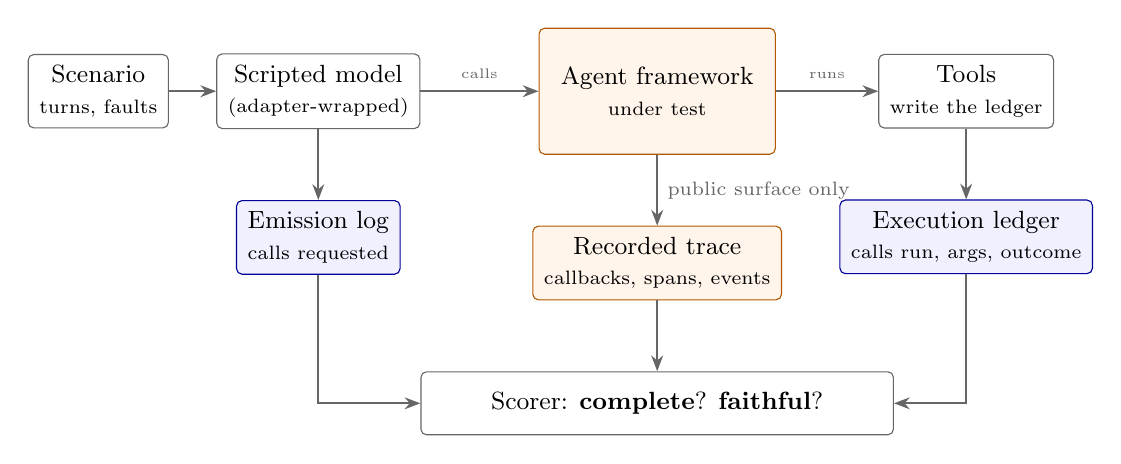
\begin{tikzpicture}[
  font=\small,
  box/.style={draw=black!60, rounded corners=2pt, minimum height=8mm, align=center, inner sep=4pt, fill=white},
  gt/.style={box, draw=blue!60!black, fill=blue!6},
  fw/.style={box, draw=orange!70!black, fill=orange!8},
  arr/.style={-{Stealth[length=2mm]}, thick, black!60},
]
\node[box] (script) {Scenario\\\scriptsize turns, faults};
\node[box, right=6mm of script] (model) {Scripted model\\\scriptsize (adapter-wrapped)};
\node[fw, right=15mm of model, minimum width=30mm, minimum height=16mm] (frame) {Agent framework\\\scriptsize under test};
\node[box, right=13mm of frame] (tools) {Tools\\\scriptsize write the ledger};
\node[gt, below=9mm of model] (em) {Emission log\\\scriptsize calls requested};
\node[gt, below=9mm of tools] (led) {Execution ledger\\\scriptsize calls run, args, outcome};
\node[fw, below=9mm of frame] (rec) {Recorded trace\\\scriptsize callbacks, spans, events};
\node[box, below=9mm of rec, minimum width=60mm] (score) {Scorer: \textbf{complete}? \textbf{faithful}?};
\draw[arr] (script) -- (model);
\draw[arr] (model) -- node[above=1pt, font=\tiny]{calls} (frame);
\draw[arr] (frame) -- node[above=1pt, font=\tiny]{runs} (tools);
\draw[arr] (model) -- (em);
\draw[arr] (tools) -- (led);
\draw[arr] (frame) -- node[right, font=\scriptsize]{public surface only} (rec);
\draw[arr] (em) |- (score);
\draw[arr] (led) |- (score);
\draw[arr] (rec) -- (score);
\end{tikzpicture}
\caption{TraceGap. Ground truth (blue) is written by the scripted model and by the tools themselves; the framework's own record (orange) is read only through its public observability surface. The scorer compares the three logs.}
\label{fig:overview}
\end{figure}

% =====================================================================
\section{Related work}
\label{sec:related}

We searched systematically for prior work in October 2026, with twelve queries including ``agent observability benchmark'', ``LLM tracing benchmark'', ``OpenTelemetry LLM benchmark'', ``agent provenance benchmark'', ``tool call tracing evaluation'', ``LLM trace completeness'' and ``agent execution provenance dataset''; the queries, inclusion criteria and per-candidate assessment are released with the benchmark. We found no benchmark or dataset that compares what agent frameworks record about tool calls with what executed, using ground truth independent of the framework.

\paragraph{Tool-use and agent benchmarks} score the model: tool selection and arguments~\citep{patil2023gorilla,qin2024toolllm} or task success in environments~\citep{yao2024tau,liu2024agentbench}. They take the framework's execution and its record for granted.

\paragraph{Work that consumes traces.} TRAIL annotates 148 OpenInference traces with agent reasoning, execution and planning errors~\citep{deshpande2025trail}; Who\&When and MAST attribute failures in multi-agent systems from their logs~\citep{zhang2025whowhen,cemri2025mast}. These label errors \emph{of the agent} and treat the trace as given. A survey of evidence tracing and execution provenance describes the area as fragmented and lists unified trace schemas as an open problem~\citep{wang2026survey}. AgentTrace proposes a structured logging layer~\citep{alsayyad2026agenttrace}, and fault-injection work uses OpenTelemetry to study how injected delays propagate through multi-agent systems~\citep{seyedghorban2026fault}. None tests whether the record itself is correct.

\paragraph{Datasets of agent traces.} AgentSec provides 30 synthetic scenarios with tool calls and W3C PROV graphs for auditing reasoning consistency~\citep{hmimou2026agentsec}. Its traces are generated from specifications rather than recorded by frameworks, so recording defects cannot arise in it.

\paragraph{Evidence that recording fails.} Zhu et al.\ classify 998 bug reports from LangChain and CrewAI and attribute 32 to ``telemetry malfunction''~\citep{zhu2026bugs}. Qin et al.\ show that agents can delete or alter their own traces when incentivized~\citep{qin2026tamper}, an adversarial counterpart to the honest recording errors studied here. Both argue for records that do not depend on the component being audited, which is how TraceGap obtains ground truth. The OpenTelemetry GenAI conventions and OpenInference define span formats for tool execution~\citep{otel2026genai,openinference2026} but come with no correctness suite for agent frameworks; TraceGap reads both.

\paragraph{Methodology.} Our benchmark validation borrows mutation testing from software engineering~\citep{demillo1978hints}: a measurement instrument is trusted when it detects deliberately injected faults. Uncertainty is quantified with the bootstrap~\citep{efron1993bootstrap} and ranking agreement with Kendall's $\tau$~\citep{kendall1938tau}. The dataset is documented with a datasheet~\citep{gebru2021datasheets}.

% =====================================================================
\section{The TraceGap benchmark}
\label{sec:method}

\subsection{Ground truth}
A \emph{case} is a scenario run on one trace surface in one execution mode. It produces two logs that do not depend on the framework:
\begin{itemize}
\item the \textbf{emission log} $E$: every tool call the scripted model returned, with its call id, name, arguments, run and nesting level;
\item the \textbf{execution ledger} $L$: every tool call that started, written from inside the tool body, with its real arguments and a final status in $\{\textsf{ok}, \textsf{error}, \textsf{cancelled}, \textsf{running}\}$, output and error message.
\end{itemize}
Every tool takes a unique \texttt{tag} argument, so records are matched to ground truth without trusting framework-assigned identifiers; surfaces that do not record arguments are matched by the model's call id. The framework's \textbf{recorded trace} $R$ is read only through its public observability interface and normalized to records $(\text{name}, \text{args}, \text{status}, \text{output}, \text{error}, \text{call id}, \text{group})$, where \emph{group} is the run identity the surface reports (a trace id, a root run id, a result object). Recorded statuses are \textsf{ok}, \textsf{error}, \textsf{incomplete} or \textsf{unknown}.

\subsection{Scripted models and adapters}
An adapter wraps a shared script cursor in the framework's own model interface, using the framework's test model where one exists, builds an agent with the scenario's tools, runs it, and converts what the surface reported into records. Adapters never rebuild events from the ledger and never patch framework internals. Each surface declares which fields it captures, and is scored only on those. Two rules keep comparisons fair. When a framework asks the model for a tool-less final answer (for example after a turn limit), the scripted model answers in text without consuming the script, as a real model offered no tools would. A case in which no call was emitted is a harness error, never a pass; this guard caught several adapter and compatibility bugs during development. The single-call scenario S01 serves as a calibration case: a surface that fails it is not being read correctly.

\subsection{Metrics}
Let $L_{\text{run}} \subseteq L$ be the calls that started, $E \setminus L$ the calls that were requested but never started (rejected by the framework, or never reached), and $m(\cdot)$ the matching from ledger and emission entries to records. A case is \textbf{complete} when all of the following hold:
\begin{enumerate}[label=(C\arabic*)]
\item \emph{recall}: every $\ell \in L_{\text{run}}$ has a record;
\item \emph{honest status}: no record of a call whose ledger status is \textsf{error}, \textsf{cancelled} or \textsf{running}, or that never ran, says \textsf{ok}; a record of a successful call is not \textsf{error}, and \textsf{incomplete} is accepted only for a call that did not finish;
\item \emph{attempt visibility}: every $e \in E \setminus L$ is visible as a record;
\item \emph{no phantoms or duplicates}: every record matches an emitted call, and no call is recorded more often than it executed;
\item \emph{isolation}: no group mixes records of two runs, and no run is split across unrelated groups.
\end{enumerate}
A case is \textbf{faithful} when every captured argument, output and error message matches the ledger exactly (outputs may be serialized; truncation is a failure). We additionally report, without scoring it, any tool still running after its run ended.

\paragraph{An observability contract, not a verdict on design.} Together, completeness and fidelity form TraceGap's \emph{observability contract}: what a consumer of a tool-level trace needs in order to reconstruct what happened. A surface that does not meet it is \emph{incomplete under the contract}, which is not the same as being wrong. Some frameworks deliberately keep rejected calls out of their tool layer, or redact errors for privacy; the contract reports the consequence for consumers without judging the choice. We call behavior a \emph{defect} only where it contradicts the surface's own semantics or the project treats it as a bug, as when a call that was cancelled is reported as successful (\S\ref{sec:fixes}). Throughout, ``complete'' and ``incomplete'' are meant in this sense.

\subsection{Scenarios}
The \textbf{core suite} has 22 hand-written scenarios in seven categories (Appendix~\ref{app:scenarios}): basic accounting (single, sequential, five parallel calls, a 25-turn session); tool failures (one raising call, failure then retry, one failure in a parallel batch); rejected calls (unknown tool, wrong argument type, missing argument); duplicate provider call ids; payload fidelity (unicode, a 200{,}000-character output, a dict, \texttt{None}, a synchronous tool); interruption (cancellation during a tool, cancellation after tools, a provider error, a turn limit); and structure (two concurrent runs, an agent nested as a tool). Cancellation uses \texttt{asyncio.Task.cancel()}, the mechanism behind timeouts and dropped requests.

The \textbf{generator} composes the same primitives into random but reproducible scenarios: one to five turns of one to four calls drawn from ten weighted call kinds (two kinds of successful call, raising, unknown tool, wrong type, missing argument, large output, structured output, \texttt{None} output, synchronous), one of five endings (final answer, cancellation in a tool, cancellation while the model thinks, provider error, turn limit), and with some probability two concurrent runs or a nested agent. Timing-dependent endings keep generous margins. A suite is identified by $(n, \text{seed})$; the released suite is $n{=}200$, seed 1, with \genCalls{} calls. Every scenario runs in \emph{invoke} and \emph{stream} mode.

\subsection{Stable and Stress tiers}
\label{sec:tiers}
A ranking that changes when the benchmark is rerun is of little use. We therefore split scenarios by a structural rule that is known before a scenario runs: a scenario is \textbf{Stress} when any model turn emits two or more calls and at least one of them raises; otherwise it is \textbf{Stable}. How a framework handles the siblings of a failing call (whether they started, finished or were recorded before the run aborted) can depend on scheduling. One core scenario (S07) and 118 of the 200 generated scenarios are Stress. Each surface has 206 Stable and 238 Stress cases across both suites and modes. The leaderboard ranks surfaces on Stable cases only, CI usage defaults to them, and Stress results are reported separately. Section~\ref{sec:validation} tests the rule on runs made after it was fixed.

% =====================================================================
\section{Validating the benchmark}
\label{sec:validation}

\paragraph{Reference loop.} A deliberately correct agent loop of about 100 lines (record the attempt before validating or executing; close the record on every exit path; never drop a requested call; tag every record with its run) is complete and faithful on all 44 core and all 400 generated cases. A perfect score is achievable, so failures reflect the surface rather than an impossible standard.

\paragraph{Mutation testing.} We injected eleven recording defects into the reference loop one at a time and ran both suites (Table~\ref{tab:mutation}). Every defect is detected, by the scenarios designed for it and on the intended axis: truncation and lost error detail are fidelity failures but not completeness failures, while dropped or misreported calls are completeness failures. On the generated suite every defect is detected in at least \mutGenMin{} of 400 cases, so the generator exercises each check without hand-written targeting. These checks, together with a negative control for every scorer check, run in the test suite.

\begin{table}[t]
\centering\small
\begin{tabularx}{\linewidth}{lXlcc}
\toprule
Injected defect & What the loop does wrong & Core scenarios detecting & Axis & Generated \\
\midrule
\inputtable{gen/tab_mutation.tex}
\bottomrule
\end{tabularx}
\caption{Mutation testing. Each defect is injected alone into the reference loop. Axis: C completeness, F fidelity. Generated: cases (of 400) where the defect is detected. Without defects the loop is complete and faithful on every case of both suites.}
\label{tab:mutation}
\end{table}

\paragraph{Why two sources of ground truth.} To test whether the emission log and the execution ledger are both necessary, we re-scored every current-release case with only one of them (Table~\ref{tab:gt}). With the emission log alone, a scorer knows what was requested but not what ran or how it ended: it catches \eoDetected{} of the \gtIncomplete{} incomplete cases (\eoDetectedPct\%), misses every case whose only failure is a dishonest status, and cannot tell a call that ran and was dropped from one that never ran, which is ambiguous in \eoAmbig{} cases. With the ledger alone, a scorer knows what ran but not what was requested, and faces a dilemma over records of calls it never saw. Treated strictly, as phantoms, they cause false alarms on \loFalse{} of the \gtComplete{} complete cases (\loFalsePct\%), because a surface that correctly records a rejected call appears to report a call that never happened; this scorer catches \loDetected{} incomplete cases (\loDetectedPct\%). Treated leniently, accepted unless they claim success, they cause only \llFalse{} false alarms, but the scorer then catches just \llDetected{} (\llDetectedPct\%) and misses every case whose only failure is an invisible attempt. Only the combination of both sources gives verdicts that are both sensitive and specific. (The handful of false alarms for the single-source scorers come from duplicate call ids in one surface, where records cannot be matched to calls without both logs.)

\begin{table}[t]
\centering\small
\begin{tabularx}{\linewidth}{lccX}
\toprule
Ground truth used & Incomplete cases detected & False alarms & What is lost \\
\midrule
\inputtable{gen/tab_gt_ablation.tex}
\bottomrule
\end{tabularx}
\caption{Ground-truth ablation on the \gtCases{} current-release cases (\gtIncomplete{} incomplete according to the full scorer, which defines the reference, so its row is correct by construction). False alarms: complete cases a single-source scorer would flag.}
\label{tab:gt}
\end{table}

\paragraph{Stability (RQ3).} All \coreCases{} core verdicts were identical across four full runs (the last two are released). Three full runs of the generated suite, all released, agreed on \stableAgree{} of \genCases{} verdicts (\stableAgreePct\%). The Stress rule was fixed after the first two generated runs, in which 104 verdicts differed, all inside it. The third run, made afterwards, added 44 differing verdicts, again all inside it: \nUnstable{} in total (119 for Pydantic AI's history, 18 for its OpenTelemetry spans, 11 for LangGraph). In every one, a call in a parallel batch raises and the framework's handling of the sibling calls is a race: in Pydantic AI, whether a sibling's result is recorded before the run aborts; in LangGraph, whether a sibling had started. Stable verdicts (\stableCases{} cases) were identical in every run.

\paragraph{Uncertainty.} Scenarios are a sample from a space of possible scenarios, so we report 95\% bootstrap confidence intervals for each surface's Stable completeness, resampling the \bootScenarios{} Stable scenarios with both modes kept together (\bootReps{} replicates; Figure~\ref{fig:ci}). Intervals are 11--18 points wide for every surface except CrewAI's events, which is complete in every case. Of the \nAdj{} adjacent pairs in the ranking, \nAdjSig{} are separated in at least 95\% of replicates: \adjSigList. The leaderboard should therefore be read as ordered groups rather than a strict order; Table~\ref{tab:main} prints the intervals beside each rank for this reason.

\paragraph{Agreement across suites.} Rankings on the core and generated Stable cases agree with Kendall $\tau = \tauCoreGen$, although the suites share no scenario. We also generated 2 further suites with different seeds ($n{=}100$; seeds 2, 3) and ran them on all surfaces. Stable-tier rankings on the 3 independently generated suites agree with Kendall $\tau$ between 0.77 and 0.80 (mean 0.78; Appendix~\ref{app:seeds}), so the ranking is not an artifact of one sample of scenarios.


\begin{figure}[t]
\centering
\begin{minipage}[t]{0.49\linewidth}
\centering
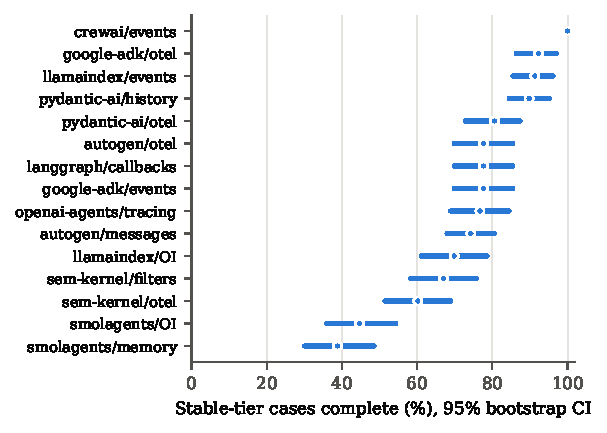
\includegraphics[width=\linewidth]{figures/fig_ci.pdf}
\caption{Stable-tier completeness per surface with 95\% bootstrap confidence intervals (scenario resampling).}
\label{fig:ci}
\end{minipage}\hfill
\begin{minipage}[t]{0.49\linewidth}
\centering
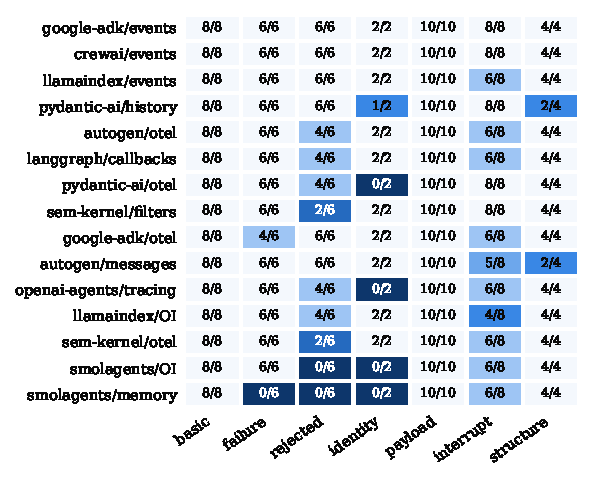
\includegraphics[width=\linewidth]{figures/fig_categories.pdf}
\caption{Complete cases per scenario category in the core suite (both modes). Darker cells mean more incomplete cases.}
\label{fig:categories}
\end{minipage}
\end{figure}

% =====================================================================
\section{Results (RQ1, RQ2)}
\label{sec:results}

We evaluate LangGraph 1.2.12, the OpenAI Agents SDK 0.23.1, Pydantic AI 2.54.0, AutoGen 0.7.5, smolagents 1.26.0, LlamaIndex 0.14.25, Semantic Kernel 1.44.1, Google ADK 2.11.0 and CrewAI 1.15.23 on Python 3.13, reading fifteen surfaces (Appendix~\ref{app:surfaces}). Table~\ref{tab:main} gives the leaderboard. Across both suites, \stableComplete{} of \stableCases{} Stable cases (\stablePct\%) and \stressComplete{} of \stressCases{} Stress cases (\stressPct\%) were complete; on the core suite alone \coreComplete{} of \coreCases{} (\corePct\%), and on the generated suite \genComplete{} of \genCases{} (\genPct\%). One surface, CrewAI's event bus, is complete and faithful on every case. This should not be read as a general claim about CrewAI's observability stack: TraceGap evaluates the selected surface on the fields it exposes, and CrewAI's events are attributed to runs by task id, information the application has, which makes the isolation criterion easier for this surface than for those that must report run identity themselves. A full run of both suites on all surfaces takes about \totalMinutes{} minutes of wall-clock time without API keys or network (Appendix~\ref{app:cost}).

\begin{table}[t]
\centering\small
\setlength{\tabcolsep}{3.6pt}
\resizebox{\linewidth}{!}{\begin{tabular}{rlcccccccccc}
\toprule
 & & \multicolumn{6}{c}{Stable tier (ranked)} & Stress & \multicolumn{2}{c}{Complete per suite} & \\
\cmidrule(lr){3-8}\cmidrule(lr){10-11}
\# & Surface & Complete \% [95\% CI] & Faithful \% & Fail. & Canc. & Rej. & Nest. & Complete \% & Core & Gen. & Fail$\to$ok \\
\midrule
\inputtable{gen/tab_leaderboard.tex}
\bottomrule
\end{tabular}}
\caption{Leaderboard. Stable tier: 206 cases per surface from both suites and modes. Capability columns count complete Stable cases among the core scenarios for tool failures (S05--S06), cancellation (S17--S18), rejected calls (S08--S10) and nested agents (S22). Fail$\to$ok: failed or cancelled calls recorded as successful (both suites).}
\label{tab:main}
\end{table}

\subsection{Where traces fall short}
\label{sec:where}
Figure~\ref{fig:categories} breaks the core suite down by category. Basic accounting and payload scenarios are complete on every surface; rejected calls (30 of the 74 incomplete core cases) and interruption (23) account for most failures, followed by duplicate call ids (9), tool failures (8) and structure (4). To separate the contributions of conditions that co-occur in generated scenarios, Table~\ref{tab:conditions} compares completeness with and without each condition and fits a logistic regression of completeness on all conditions, the log number of calls and surface fixed effects. Rejected calls ($\beta$\,=\,\logitRej), parallel calls (\logitPar), cancellation (\logitCanc) and a raising tool (\logitRaise) have the largest effects, followed by nested agents (\logitNest); once these are accounted for, provider errors, turn limits and concurrent runs have little effect on average, though they matter for specific surfaces (\S\ref{sec:failures}). Completeness also falls with scenario size (log-calls coefficient \logitCalls): pooled over surfaces, from \curveLo\% for scenarios with one to three calls to \curveHi\% for those with sixteen or more (Figure~\ref{fig:calls}). The decline is surface-specific: Google ADK's spans stay near 100\%, LangGraph's callbacks stay flat, and smolagents' memory falls from \smolLo\% to \smolHi\%, because a single failing call removes every call of its step.

\begin{table}[t]
\centering\small
\begin{tabular}{lcccc}
\toprule
Condition (generated suite) & Scenarios & \% complete with & \% complete without & Logit coef. \\
\midrule
\inputtable{gen/tab_conditions.tex}
\bottomrule
\end{tabular}
\caption{Completeness on the generated suite (all fifteen surfaces, 6{,}000 cases) by condition. The logistic regression includes all conditions except the Stress indicator (which is their conjunction), the log number of calls and surface fixed effects.}
\label{tab:conditions}
\end{table}

\begin{figure}[t]
\centering
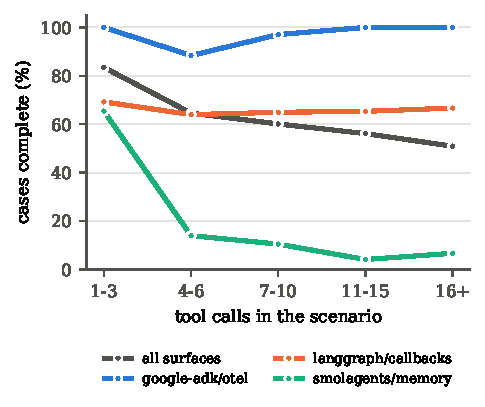
\includegraphics[width=0.5\linewidth]{figures/fig_calls.pdf}
\caption{Completeness against the number of tool calls in a generated scenario, pooled over all surfaces and for three surfaces with different behavior.}
\label{fig:calls}
\end{figure}

\subsection{Why the criteria matter: a metric ablation}
The obvious first metric for a trace is recall: does every executed call appear? Of the \ablIncomplete{} incomplete cases across both suites, \ablRecallMiss{} (\ablRecallMissPct\%) have no missing executed call and would pass a recall-only check. Adding honest status still passes \ablRSMiss{} of them (\ablRSMissPct\%). The dominant failure is invisible attempts (\ablInvisible{} cases, \ablInvisibleOnly{} with no other failure): the model asked for a call, the framework rejected it before execution, and the tool-level trace says nothing. Missing executed calls occur in \ablMissing{} cases, wrong statuses other than false success in \ablStatus{}, and false success in \ablFalseOk{}. A trace validator that only counts spans would therefore report most incomplete traces as healthy. No case in the corpus fails the phantom, duplicate or isolation checks; they are exercised by the injected defects (Table~\ref{tab:mutation}), which fail them.

\subsection{Failure modes}
\label{sec:failures}
\begin{figure}[t]
\centering
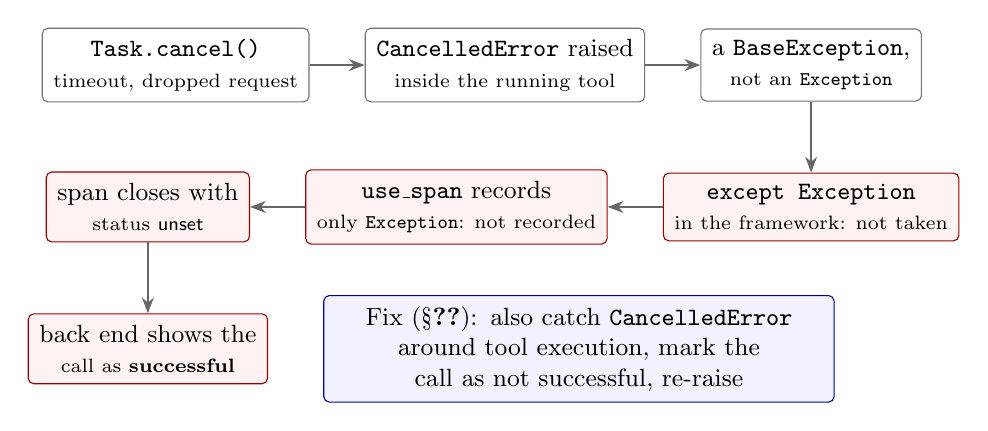
\begin{tikzpicture}[font=\small,
  st/.style={draw=black!55, rounded corners=2pt, align=center, inner sep=4pt, fill=white, minimum height=7mm},
  bad/.style={st, draw=red!60!black, fill=red!5},
  ok/.style={st, draw=blue!60!black, fill=blue!5},
  arr/.style={-{Stealth[length=2mm]}, thick, black!60}]
\node[st] (cancel) {\texttt{Task.cancel()}\\\scriptsize timeout, dropped request};
\node[st, right=7mm of cancel] (raise) {\texttt{CancelledError} raised\\\scriptsize inside the running tool};
\node[st, right=7mm of raise] (base) {a \texttt{BaseException},\\\scriptsize not an \texttt{Exception}};
\node[bad, below=9mm of base] (miss) {\texttt{except Exception}\\\scriptsize in the framework: not taken};
\node[bad, left=7mm of miss] (otel) {\texttt{use\_span} records\\\scriptsize only \texttt{Exception}: not recorded};
\node[bad, left=7mm of otel] (close) {span closes with\\\scriptsize status \textsf{unset}};
\node[bad, below=9mm of close] (ui) {back end shows the\\\scriptsize call as \textbf{successful}};
\node[ok, right=7mm of ui, text width=62mm] (fix) {Fix (\S\ref{sec:fixes}): also catch \texttt{CancelledError} around tool execution, mark the call as not successful, re-raise};
\draw[arr] (cancel) -- (raise);
\draw[arr] (raise) -- (base);
\draw[arr] (base) -- (miss);
\draw[arr] (miss) -- (otel);
\draw[arr] (otel) -- (close);
\draw[arr] (close) -- (ui);
\end{tikzpicture}
\caption{Why cancelled tool calls look successful. Semantic Kernel and Google ADK follow this path through \texttt{use\_span}; the OpenAI Agents SDK's own span context manager has the same blind spot; AutoGen shows it once its orphaned-tool defect is fixed (\S\ref{sec:fixes}).}
\label{fig:cancel}
\end{figure}

\paragraph{Cancellation is reported as success.} OpenTelemetry's \texttt{use\_span} records only \texttt{Exception}, and \texttt{asyncio.CancelledError} is a \texttt{BaseException}. A framework that wraps tool execution in \texttt{except Exception} therefore closes a cancelled tool's span with an unset status, which back ends display as success (Figure~\ref{fig:cancel}). We observed this in the OpenAI Agents SDK, whose own span context manager ignores the exception type, and in Semantic Kernel and Google ADK; ADK is also affected when it cancels the siblings of a failed parallel call, and AutoGen shows it once its orphaned-tool defect is fixed. Pydantic AI handles cancellation explicitly. Separately, cancellation does not always stop work: AutoGen, LlamaIndex, smolagents and CrewAI let an in-flight tool finish after the caller has seen the run cancelled.

\paragraph{Failed runs lose completed calls.} AutoGen's \texttt{TaskResult.messages} exists only when a run completes, though its \texttt{run\_stream()} events keep the calls. When one call in a parallel batch raises, Google ADK's events and Pydantic AI's history drop the results of siblings that succeeded, which is why ADK's events score 77.7\% on Stable cases but 14.3\% on Stress cases while its spans score 99.2\% on Stress. smolagents' memory drops every call of a step in which any call failed.

\paragraph{Rejected calls and nesting.} A call to an unknown tool, or with invalid arguments, is often visible only in raw model output. Calls made by an agent used as a tool are missing from the per-agent histories of Pydantic AI and AutoGen, but present in their tracing and OpenTelemetry surfaces.

\paragraph{Fidelity.} Across Stable cases \stableFaithful{} of \stableCases{} (\stableFaithfulPct\%) are faithful. Arguments were recorded exactly by every surface that records them. Error details are the main gap: the OpenAI Agents SDK redacts tool errors from spans under its default error handler, deliberately and for privacy, and Google ADK's events and Pydantic AI's history keep no error when a tool raises; ADK's events also omit some outputs.

% =====================================================================
\section{Defects and fixes}
\label{sec:fixes}

\begin{table}[t]
\centering\small
\begin{tabularx}{\linewidth}{lXl}
\toprule
Project & Defect & Scenarios \\
\midrule
OpenAI Agents SDK & cancelled function span has no error & S17 \\
AutoGen & \texttt{run()} hangs after a \texttt{CancellationToken} cancel during a tool; the in-flight tool keeps running after task cancel; once that is fixed, the cancelled tool span is unset & S17 \\
Semantic Kernel & cancelled function span unset (\texttt{invoke}, \texttt{invoke\_stream}) & S17 \\
Google ADK & cancelled tool span unset, including cancelled parallel siblings & S07, S17 \\
smolagents & step memory loses all tool calls when one fails; duplicate call ids silently dropped (reported, not patched) & S05--S07, S11 \\
\bottomrule
\end{tabularx}
\caption{Defects found by TraceGap.}
\label{tab:fixes}
\end{table}

For each defect in Table~\ref{tab:fixes} we wrote a minimal fix against the project's main branch, with a regression test that fails before the fix and passes after; the surrounding test suites show no new failures, and the affected TraceGap scenarios pass on the patched framework. Table~\ref{tab:upstream} lists what is released for each finding.

\begin{table}[h]
\centering\small
\begin{tabularx}{\linewidth}{llX}
\toprule
Project & Finding & Released with the benchmark \\
\midrule
OpenAI Agents SDK & cancelled function span has no error & patch, regression test, standalone reproduction \\
AutoGen & cancellation hang, orphaned tool, unset span & patch, regression tests, standalone reproductions \\
Semantic Kernel & cancelled function span unset & patch, regression test \\
Google ADK & cancelled tool spans unset & patch, regression test \\
smolagents & failed step loses calls; duplicate ids dropped & patch and regression test (lost calls); scenario S11 (duplicate ids) \\
\bottomrule
\end{tabularx}
\caption{Fixes and reproductions released for each finding. Every finding is also reproduced by the TraceGap scenarios listed in Table~\ref{tab:fixes}.}
\label{tab:upstream}
\end{table}

% =====================================================================
\section{History across releases (RQ4)}
\label{sec:history}

Because the models are scripted, the same suite can be run against past releases. We ran the core suite against 69 releases published between \histFirst{} and \histLast{}, installing each with dependencies resolved as of one day after its release (\texttt{uv --exclude-newer}), so each run sees what users installed at the time. Four old Semantic Kernel releases needed current resolution because their original dependency set no longer installs. Of the 69 releases, 65 ran; one had a dependency mismatch, one used an older API, and two CrewAI releases supported only ReAct-style tool calling. Version--surface pairs that fail the calibration case are left out (11 pairs). Figure~\ref{fig:history} shows every surface whose core completeness changed, and Appendix~\ref{app:history} summarizes all surfaces. The history shows gaps arriving and leaving: smolagents' memory loss arrived together with parallel tool calls in 1.18.0 and its silent dropping of duplicate call ids in 1.20.0; the OpenAI Agents SDK began rejecting duplicate call ids in 0.20.0 and redacting tool errors from spans in 0.23; Pydantic AI's OpenTelemetry spans began showing rejected calls in 2.30.0, and Google ADK's spans across 2.7.1 and 2.9.2; CrewAI's events began showing calls to unknown tools in 1.15.23. Where a framework executed a scenario differently between versions (for example, emitting a different number of calls), the report says so rather than attributing the change to tracing. Run on every release, TraceGap works as a regression suite: each of these changes would have been flagged in the release that introduced it.

\begin{figure}[t]
\centering
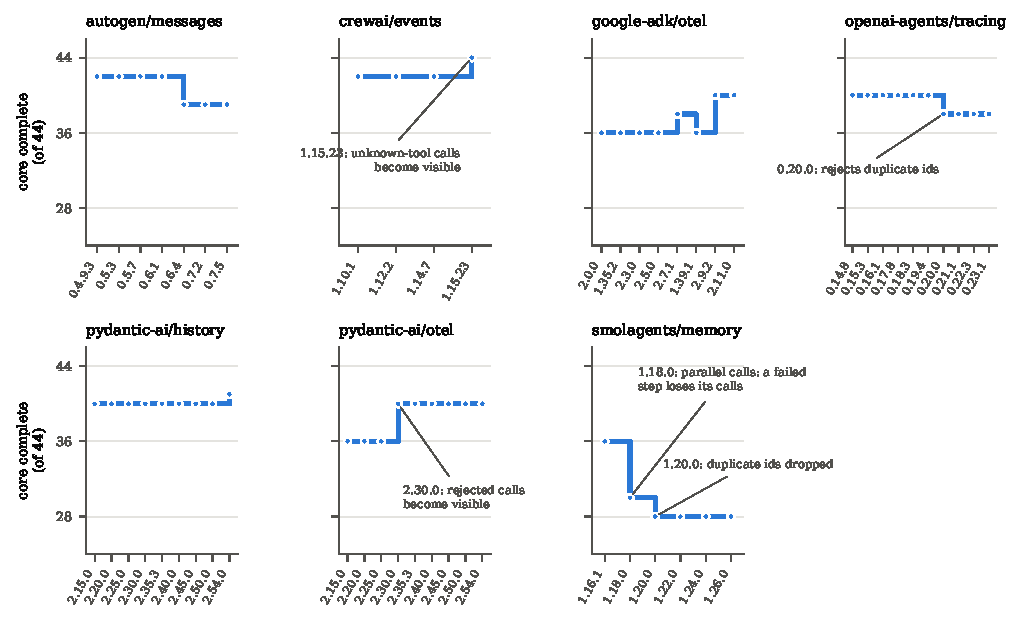
\includegraphics[width=\linewidth]{figures/fig_history.pdf}
\caption{Core-suite completeness (of 44 cases) across releases, for the seven surfaces whose completeness changed. Releases are ordered by date; Google ADK maintained 1.x and 2.x lines in parallel. Annotated changes are confirmed in the per-version verdict diffs. Some changes mix improvements and regressions (smolagents 1.18.0 fixed S03 and S11 while breaking five scenarios), and two (AutoGen 0.6.4, Pydantic AI history 2.54.0) reflect the framework executing a scenario differently rather than a tracing change.}
\label{fig:history}
\end{figure}

% =====================================================================
\section{Dataset and learning tasks (RQ5, RQ6)}
\label{sec:data}

\paragraph{Corpus.} Every case is released with its three aligned logs (emissions, ledger, recorded trace), labels, tier, the reason for each failure and per-case counters: 6{,}660 cases for current releases (core and generated) and 4{,}884 for the 65 past releases, with a calibration flag. The corpus is documented with a datasheet~\citep{gebru2021datasheets} and can be regenerated in minutes. Table~\ref{tab:dataset} summarizes its composition and Appendix~\ref{app:labels} the distribution of defect labels.

\begin{table}[t]
\centering\small
\begin{tabular}{lr}
\toprule
Property & Count \\
\midrule
\inputtable{gen/tab_dataset.tex}
\bottomrule
\end{tabular}
\caption{Composition of the released corpus (current and past releases).}
\label{tab:dataset}
\end{table}

\paragraph{Tasks.} Because each recorded trace is paired with what really ran, the corpus can evaluate methods that analyse traces, such as trace validators, observability back ends and LLM-based judges. We define tasks that hide the ledger and give a method what a real pipeline sees: the emitted calls, the recorded trace and the run's outcome. The harness's unique \texttt{tag} is removed from the inputs, both as a field and as an argument inside emitted and recorded calls, because production tools have no such argument; calls can be joined only by call id, or by name and the remaining arguments. Tag values that some tools echo in their outputs or error messages are replaced by a placeholder. (The scorer still uses tags; only the learning inputs are masked.)
\begin{itemize}
\item \textbf{T1 Completeness detection} (binary): is the trace complete?
\item \textbf{T2 Fidelity detection} (binary): are its arguments, outputs and errors exact?
\item \textbf{T3 Defect classification} (multi-label over ten types): missing call, invisible attempt, false success, other status mismatch, duplicate, phantom, isolation, lost arguments, lost output, lost error. Labels are derived mechanically from the scorer's failure reasons.
\item \textbf{T4 Execution reconstruction}: for each emitted call, was it \textsf{ok}, \textsf{error}, \textsf{cancelled}, still \textsf{running}, or never executed?
\end{itemize}
A fifth task, converting a framework's native trace into the canonical record, is the adapter task and is scored by the benchmark itself. Splits hold out whole frameworks, so methods must generalize to unseen trace conventions: train (LangGraph, Pydantic AI, AutoGen, LlamaIndex, CrewAI; \taskTrainN{} examples), validation (OpenAI Agents SDK, Semantic Kernel; \taskValN) and test (Google ADK, smolagents; \taskTestN). Uncalibrated rows and harness errors are excluded.

\paragraph{Baselines.} We evaluate six methods. A \emph{majority-class} baseline; a \emph{rule-based} baseline that matches emitted to recorded calls by call id and, failing that, one-to-one by name and arguments, and applies rules an engineer could write without the ledger; \emph{logistic regression} and \emph{gradient-boosted trees}~\citep{pedregosa2011sklearn} on 24 hand-designed, surface-agnostic case-level features (counts of emitted, recorded and unmatched calls, recorded statuses, missing outputs and errors, emitted calls that violate the tool schema, run structure, run outcome and mode) and, for T4, 16 call-level features plus the 24 case-level features of the call's case; two further features, the rates at which a surface captures arguments and call ids, characterize a surface's conventions and are evaluated separately below because they hurt generalization; and two models that read the trace as a token sequence: \emph{TF-IDF n-grams with logistic regression} and a small \emph{transformer encoder} trained from scratch (Appendix~\ref{app:sequence}). Inputs come from task fields only; tool schemas are treated as known, as they are to any real pipeline, but tool \emph{names} are not used, since the benchmark's names (such as \texttt{fail}) reveal behavior that real names would not. T3 uses one binary output per label. The sequence models address T1--T3; T4 uses the feature models.

\begin{table}[t]
\centering\small
\resizebox{\linewidth}{!}{%
\begin{tabular}{lcccccc}
\toprule
 & \multicolumn{2}{c}{T1 completeness} & \multicolumn{2}{c}{T2 fidelity} & \multicolumn{2}{c}{T3 defects} \\
\cmidrule(lr){2-3}\cmidrule(lr){4-5}\cmidrule(lr){6-7}
Method (test: Google ADK, smolagents) & F1 & Bal.\ acc. & F1 & Bal.\ acc. & Micro F1 & Macro F1 \\
\midrule
\inputtable{gen/tab_tasks_all.tex}
\bottomrule
\end{tabular}}
\caption{RQ5: detection without the ledger, on the held-out test frameworks. F1 treats the defect (incomplete, unfaithful) as the positive class. Sequence models: mean $\pm$ standard deviation over three training seeds (TF-IDF is deterministic).}
\label{tab:tasks}
\end{table}

\begin{table}[t]
\centering\small
\resizebox{\linewidth}{!}{%
\begin{tabular}{lccccccccc}
\toprule
 & \multicolumn{3}{c}{T1 F1} & \multicolumn{3}{c}{T2 F1} & \multicolumn{3}{c}{T3 macro F1} \\
\cmidrule(lr){2-4}\cmidrule(lr){5-7}\cmidrule(lr){8-10}
Method & Random & Held-out & LOFO & Random & Held-out & LOFO & Random & Held-out & LOFO \\
\midrule
\inputtable{gen/tab_splits.tex}
\bottomrule
\end{tabular}}
\caption{RQ6: the same methods under three evaluation protocols. Random: 80/20 split of all cases, every framework seen in training (mean $\pm$ s.d.\ over five split seeds for feature models, three for sequence models). Held-out: the official split. LOFO: leave one framework out, mean $\pm$ population s.d.\ across held-out frameworks that have positive cases for the task (nine for T1 and T3, three for T2); the transformer is trained once per fold.}
\label{tab:splits}
\end{table}

\paragraph{Detection is largely learnable (RQ5).} Table~\ref{tab:tasks} shows that whether a trace is complete can be predicted well from what a pipeline already has: gradient-boosted trees on simple features reach F1 \gbmTOneF{} on T1 for frameworks never seen in training. Fidelity loss (T2) is highly detectable in this corpus, largely through status-related features (see below), and its cross-framework evidence is limited to three framework families. The rule-based baseline, which encodes the natural assumption that an absent call never ran, does markedly worse, and on T4 it is below the majority class in call accuracy (Table~\ref{tab:t4}) because smolagents' memory drops whole steps that did execute and Google ADK's events drop the results of calls that completed. Characterizing \emph{what} was lost is harder: macro F1 on T3 stays well below detection accuracy for every method. The sequence models, which must discover the relevant structure themselves, trail the hand-designed features; the transformer reaches T1 F1 \seqTOneHeld{} and T3 macro F1 \seqTThreeHeld{}.

\paragraph{Random splits overestimate generalization (RQ6).} Table~\ref{tab:splits} evaluates every learned method under three protocols. For all four methods and all three tasks, the leave-one-framework-out average is below the random-split score, by \dropMin{} to \dropMax{}, and it varies widely across held-out frameworks (standard deviation up to \lofoSdMax). For gradient-boosted trees, T3 macro F1 is \iidGbmTThreeMean{} on a random split but \gbmTThreeMacro{} on the official held-out split and \lofoGbmTThreeMean{} averaged over LOFO folds; T4 case exact match falls from \iidTFourExact{} to \gbmTFourExact{} (Table~\ref{tab:t4}). The official test split is itself easier than the LOFO average on T1 and T2 for every method, and on T2 it scores even higher than the random split; a single held-out split can therefore also be optimistic, and LOFO with its spread is the more reliable protocol. Per-framework results (Table~\ref{tab:lofo}) show why: frameworks fail in different ways (smolagents drops steps, Google ADK drops sibling results, the OpenAI Agents SDK withholds errors), and a detector learns the failure modes it has seen. A random split, which places cases from the same framework, version and scenario on both sides, therefore overstates how well a trace validator will work on a new framework. We recommend that work on this corpus report LOFO results with their spread. Inferring \emph{how} an unseen framework fails from what its trace omits is the open problem the tasks pose.

\paragraph{T2 is preliminary across frameworks.} Fidelity failures occur in only three framework families (Google ADK, Pydantic AI and the OpenAI Agents SDK), so T2's LOFO average rests on three folds, and its large spread (up to $\pm$\lofoSdMax) reflects limited support rather than instability of the method. We treat cross-framework conclusions about T2 as preliminary.

\paragraph{Are the features shortcuts?} Two threats deserve direct tests: that hand-designed features encode the labels almost by definition, and that they let a model recognize the surface and recall its typical failures. Table~\ref{tab:featabl} adds feature groups cumulatively, starting from counts and ending with all 26 features; the reference baselines elsewhere use the surface-agnostic set (second-to-last row). Counts and structure alone already detect incompleteness on the held-out frameworks (T1 F1 \faCountsTOne). T2, in contrast, is close to definitional in this corpus: recorded statuses lift held-out T2 F1 from near zero to above .96, because most fidelity failures are error messages lost when a tool raises, which shows up as error-status records; T2 therefore measures little beyond that here. The features that most directly characterize a surface, the rates at which it captures arguments and call ids, \emph{hurt} generalization: without them, gradient-boosted trees reach LOFO T1 F1 \faNoRatesTOneLofo{} and T3 macro F1 \faNoRatesTThreeLofo, against \faAllTOneLofo{} and \faAllTThreeLofo{} with them. On the two held-out test frameworks the same change is smaller (T1 F1 \faAllTOne{} to \faNoRatesTOne, T3 macro F1 \faAllTThree{} to \faNoRatesTThree), so a single held-out split would understate it. A probe confirms that the features carry surface identity: a classifier names the surface (one of \probeClasses) with \probeAll\% accuracy from all features, \probeNoRates\% without the rates and \probeCounts\% from counts alone, against \probeChance\% for the majority class (scenario-grouped five-fold cross-validation). A detector that can recognize the surface can fall back on that surface's typical failure modes, which does not transfer to new frameworks. This is a caution for trace validators generally: features that identify the trace surface can cost little on one held-out split while hurting generalization across frameworks, which leave-one-framework-out evaluation exposes. We therefore use the surface-agnostic set for the reference feature baselines throughout.

\paragraph{Masking the harness tag.} All task results above use inputs from which the harness's tag has been removed. Table~\ref{tab:tag} compares them with unmasked inputs, using all 26 features on both sides. Masking changes the feature models' scores by at most \tagMaxDiff{} on the official split and \tagMaxDiffLofo{} in mean LOFO score, so the tag did not drive the results: matching by call id and, for calls without a usable id, one-to-one by name and the remaining arguments recovers the same information. The sequence models compare calls only through call ids and never read argument values; their inputs are identical with and without the tag (checked for all 11{,}060 examples).

\begin{table}[t]
\centering\small
\resizebox{\linewidth}{!}{%
\begin{tabular}{lrcccccccc}
\toprule
 & & \multicolumn{3}{c}{GBT, held-out split} & \multicolumn{3}{c}{GBT, LOFO (mean $\pm$ s.d.)} & \multicolumn{2}{c}{LR, held-out} \\
\cmidrule(lr){3-5}\cmidrule(lr){6-8}\cmidrule(lr){9-10}
Features (cumulative) & \# & T1 F1 & T2 F1 & T3 macro & T1 F1 & T2 F1 & T3 macro & T1 F1 & T3 macro \\
\midrule
\inputtable{gen/tab_feat_ablation.tex}
\bottomrule
\end{tabular}}
\caption{Feature ablation. The second-to-last row is the surface-agnostic model used as the reference feature baseline in Tables~\ref{tab:tasks}--\ref{tab:lofo}; the last row adds the two captured-field rates that characterize a surface's conventions.}
\label{tab:featabl}
\end{table}

\begin{table}[t]
\centering\small
\resizebox{\linewidth}{!}{%
\begin{tabular}{lcccccc}
\toprule
 & \multicolumn{4}{c}{Held-out split} & \multicolumn{2}{c}{LOFO mean} \\
\cmidrule(lr){2-5}\cmidrule(lr){6-7}
Method & T1 F1 & T2 F1 & T3 macro F1 & T4 case exact & T1 F1 & T3 macro F1 \\
\midrule
\inputtable{gen/tab_tag.tex}
\bottomrule
\end{tabular}}
\caption{Effect of masking the harness tag in task inputs: unmasked $\rightarrow$ masked.}
\label{tab:tag}
\end{table}

\begin{table}[t]
\centering\small
\begin{tabular}{lccc}
\toprule
Method & Call accuracy & Macro F1 & Case exact \\
\midrule
\inputtable{gen/tab_t4.tex}
\bottomrule
\end{tabular}
\caption{T4 execution reconstruction on the held-out test frameworks; the last row is the random-split reference (frameworks seen).}
\label{tab:t4}
\end{table}

\begin{table}[t]
\centering\small
\resizebox{\linewidth}{!}{%
\begin{tabular}{lrcccccccccc}
\toprule
 & & \multicolumn{5}{c}{T1 F1} & \multicolumn{5}{c}{T3 macro F1} \\
\cmidrule(lr){3-7}\cmidrule(lr){8-12}
Held-out framework & Examples & Rules & LR & GBT & TF-IDF & Transf. & Rules & LR & GBT & TF-IDF & Transf. \\
\midrule
\inputtable{gen/tab_lofo_t13.tex}
\bottomrule
\end{tabular}}
\caption{Leave-one-framework-out: train on eight frameworks, test on the ninth (all splits pooled; one training run per fold). CrewAI has six defective cases, all from past releases, so its F1 is near zero for most methods: with almost no positives, a few missed cases dominate the score. Per-framework F1 is therefore not a ranking of frameworks or of how hard they are.}
\label{tab:lofo}
\end{table}

\section{Discussion and limitations}
\label{sec:discussion}

Several gaps are deliberate design choices: redaction protects sensitive data, and rejecting malformed responses is reasonable. TraceGap does not judge these choices; it makes their consequences visible to people who build on the trace. The cancellation pattern is different: it follows from an interaction between OpenTelemetry's exception handling and Python's exception hierarchy that framework authors can easily miss. Whether a cancelled call should be recorded as an \emph{error} is debatable, and some maintainers deliberately keep run cancellation from marking spans; TraceGap requires only that a call that never finished does not read as a success. We suggest that the GenAI semantic conventions state how cancelled tool calls should be recorded.

For machine-learning practice the implication is direct. Trajectories exported from framework traces for evaluation or training, and trace-based judges, inherit these gaps: an evaluator reading a trace that omits rejected attempts or reports cancelled calls as successful will misjudge the agent. Our ablation suggests that span counting, the cheapest validator, misses most such traces, while the learned baselines show that incompleteness itself is detectable from what a pipeline already has.

\paragraph{Limitations.} TraceGap covers Python frameworks only. Scripted models exercise framework logic, not provider clients, so defects specific to one provider integration will not appear, and the distribution of conditions differs from natural traffic; the benchmark measures behavior under specified conditions rather than incident rates in production. Attempt visibility is judged at the tool layer; a call visible only in raw model output does not count. CrewAI's events are attributed to runs by task id, information the application has, so its isolation checks are lenient. Cancellation is applied uniformly with \texttt{asyncio.Task.cancel()}. Adapters are written by us; the calibration case, the reference loop and mutation testing guard against adapter errors but cannot rule them out, and every failure we report was confirmed by hand. Results apply to the pinned versions. The Stress rule was tested on one run of the released suite made after it was fixed; the two additionally seeded suites were run once each and support the ranking agreement, not the rule. A framework with races of a different structure would need the rule extended. Our learned baselines are deliberately simple; the transformer is trained from scratch because our environment had no access to pretrained weights, and pretrained or LLM-based trace readers are the obvious next step.

\paragraph{Broader impact.} TraceGap aims to make agent systems more accountable by checking the records that oversight relies on. Its data is synthetic and contains no personal information. Publishing framework defects could in principle inform attackers who wish to hide actions, but the defects concern honest recording and were reported upstream with fixes; records that do not depend on the audited component, as in TraceGap's ledger, are the general defense.

% =====================================================================
\section{Conclusion}
The trace an agent framework produces is infrastructure that other systems trust. TraceGap shows that this trust is mostly but not fully justified, that the gaps concentrate where an accurate record matters most, and that they can be measured reproducibly, ranked with known uncertainty, and fixed. The code, scenarios, results, fixes, corpus and tasks are released at \codeurl.

\paragraph{Reproducibility statement.} Every number in this paper is produced by scripts in the released repository from released result files; framework versions are pinned per environment; no API keys or network access are needed to rerun the benchmark. The generated suites are identified by $(n, \text{seed})$.

\paragraph{Use of AI assistance.} The benchmark software and an initial draft of this paper were developed with substantial assistance from an AI assistant (Claude, Anthropic). The author directed the work, reviewed and verified all results, and takes full responsibility for the content.

\bibliography{refs}
\bibliographystyle{tmlr}

% =====================================================================
\appendix
\section{Core scenarios}
\label{app:scenarios}
\begin{small}
\begin{tabularx}{\linewidth}{llp{3.2cm}X}
\toprule
Id & Category & Title & Description \\
\midrule
\inputtable{gen/tab_scenarios.tex}
\bottomrule
\end{tabularx}
\end{small}

\section{Trace surfaces}
\label{app:surfaces}
\begin{small}
\begin{tabularx}{\linewidth}{lX}
\toprule
Surface & What is read \\
\midrule
\texttt{langgraph/callbacks} & LangChain \texttt{on\_tool\_start/end/error} callbacks \\
\texttt{openai-agents/tracing} & \texttt{FunctionSpanData} spans via a \texttt{TracingProcessor} \\
\texttt{pydantic-ai/history} & \texttt{capture\_run\_messages()} / \texttt{run\_stream\_events()} \\
\texttt{pydantic-ai/otel} & \texttt{execute\_tool} OpenTelemetry spans \\
\texttt{autogen/messages} & \texttt{ToolCallRequest/ExecutionEvent} from \texttt{run()} / \texttt{run\_stream()} \\
\texttt{autogen/otel} & autogen-core \texttt{execute\_tool} spans (name and call id only) \\
\texttt{smolagents/memory} & \texttt{agent.memory.steps} (presence, arguments and call ids only) \\
\texttt{smolagents/openinference} & OpenInference \texttt{TOOL} spans \\
\texttt{llamaindex/events} & \texttt{ToolCall} / \texttt{ToolCallResult} workflow events \\
\texttt{llamaindex/openinference} & OpenInference \texttt{TOOL} spans \\
\texttt{semantic-kernel/filters} & a \texttt{FUNCTION\_INVOCATION} filter \\
\texttt{semantic-kernel/otel} & Semantic Kernel GenAI diagnostics spans \\
\texttt{google-adk/events} & \texttt{Runner.run\_async} events \\
\texttt{google-adk/otel} & ADK \texttt{execute\_tool} spans \\
\texttt{crewai/events} & \texttt{ToolUsageStarted/Finished/Error} on the CrewAI event bus \\
\bottomrule
\end{tabularx}
\end{small}

\section{Ranking robustness across generated suites}
\label{app:seeds}
Stable-tier completeness (\%) per surface on independently generated suites: seed 1 ($n{=}200$, the released suite) and seeds 2, 3 ($n{=}100$).

\begin{center}\small
\begin{tabular}{lccc}
\toprule
Surface & Seed 1 & Seed 2 & Seed 3 \\
\midrule
\inputtable{gen/tab_seeds.tex}
\bottomrule
\end{tabular}
\end{center}
Individual rates move by up to 16 points between suites (largest for \texttt{langgraph/callbacks}), consistent with the bootstrap intervals in Figure~\ref{fig:ci}. \texttt{crewai/events} ranks first in every suite and the same three surfaces (\texttt{semantic-kernel/otel}, \texttt{smolagents/memory}, \texttt{smolagents/openinference}) occupy the last three places in every suite.


\section{History per surface}
\label{app:history}
\begin{center}\small
\begin{tabular}{lccc}
\toprule
Surface & Versions & Release dates & Core complete (of 44) \\
\midrule
\inputtable{gen/tab_history.tex}
\bottomrule
\end{tabular}
\end{center}
Uncalibrated version--surface pairs are excluded. Per-version results and every verdict change are in the released history report.

\section{Cost}
\label{app:cost}
\begin{center}\small
\begin{tabular}{lcc}
\toprule
Surface & Median seconds per case & Total minutes (both suites) \\
\midrule
\inputtable{gen/tab_cost.tex}
\bottomrule
\end{tabular}
\end{center}
Times are wall clock on a two-core cloud machine, dominated by deliberate delays in timing scenarios.

\section{Defect labels}
\label{app:labels}
Distribution of T3 defect labels over calibrated cases of both splits (a case can carry several labels). Labels with zero count occur only under injected defects (Table~\ref{tab:mutation}).
\begin{center}\small
\begin{tabular}{lr}
\toprule
Label & Cases \\
\midrule
\inputtable{gen/tab_labels.tex}
\bottomrule
\end{tabular}
\end{center}

\section{Sequence models}
\label{app:sequence}
\paragraph{Serialization.} Each example becomes a token sequence (at most 256 tokens): a mode token; run-outcome tokens; then, for each emitted call, its position, schema validity, run index and nesting; then, for each recorded event, the position of the emitted call it refers to by call id (or an unknown marker), its status, whether output, error, arguments and call id are present, and a group index. Tool names and argument values are not used.

\paragraph{TF-IDF + logistic regression.} 1--3-gram TF-IDF over the token sequence (minimum document frequency 2, sublinear term frequency), class-balanced logistic regression with $C{=}4$, one model per binary label.

\paragraph{Transformer.} A two-layer encoder with four heads, width 64, learned positional embeddings and a \textsc{cls} token, trained from scratch in JAX with AdamW (learning rate $2\times10^{-3}$, cosine schedule with warm-up, weight decay 0.01, batch 64, 6 epochs) and a shared trunk with heads for T1, T2 and the ten T3 labels (class-weighted binary cross-entropy). Our compute environment had no access to pretrained model weights, so we train from scratch; pretrained encoders are a natural next baseline.

\section{Task features}
\label{app:features}
Case features (24 in the reference baselines, 26 in the ablation): numbers of emitted and recorded calls and their difference; share of emitted calls matched; unmatched emitted calls; emitted calls matched more than once; unmatched records; counts of recorded \textsf{ok}, \textsf{error}, \textsf{incomplete} and \textsf{unknown} statuses; emitted calls violating the tool schema, in total and among unmatched calls; unmatched schema-valid calls; \textsf{ok} records without output; \textsf{error} records without a message; shares of records without arguments and without call ids (the two surface-characterizing features, used only in the ablation); number of groups, number of runs and whether groups exceed runs; nested emitted calls; mode; and run-outcome indicators (completed, cancelled, raised). Call features (16, combined with the case features of the call's case for T4): whether and how often the call is matched; the matched record's status indicators; whether its output is missing and its error present; schema validity; nesting; relative position; whether the call comes after the last matched call of its run; whether it is last; and the run-outcome indicators.

\end{document}
